\documentclass[journal]{IEEEtran}

% \usepackage[T1]{fontenc}

\usepackage{amsfonts,bm,cite,amssymb,color,balance,graphicx,bm}

\usepackage{amsmath}
\interdisplaylinepenalty=2500
% \usepackage[cmintegrals]{newtxmath}

\ifCLASSOPTIONcompsoc
 \usepackage[caption=false,font=normalsize,labelfont=sf,textfont=sf]{subfig}
\else
 \usepackage[caption=false,font=footnotesize]{subfig}
\fi


\def \blkdiag{\operatorname{blkdiag}}
\def \diag{\operatorname{diag}}
\def \ln{\operatorname{ln}}
\def \arg{\operatorname{arg}}
\def \tr{\operatorname{tr}}

% correct bad hyphenation here
% \hyphenation{op-tical net-works semi-conduc-tor}


\begin{document}

\title{indoor DPD}

\author{Kegang~Hao,~\IEEEmembership{Student Member,~IEEE,}
        and~Qun~Wan,~\IEEEmembership{Member,~IEEE}%
\thanks{K.G. Hao and Q. Wan are with the University of Electronic Science and Technology of China, Chengdu, 611731 China e-mail: (haokegang@std.uestc.edu.cn).}% 
\thanks{This work was supported in part by the National Natural Science Foundation of China (NSFC) under Grant 61771108 and U1533125, and the Fundamental Research Funds for the Central Universities under Grant ZYGX2015Z011.}
}

\maketitle

\begin{abstract}


\end{abstract}

\begin{IEEEkeywords}


\end{IEEEkeywords}


\IEEEpeerreviewmaketitle


\section{Introduction}
\label{sec:intro}
\IEEEPARstart{M}{ultiple} \cite{Amar2004Direct} 


\section{System model and Problem formulation}
\label{sec:model and problem}
We consider a mm-wave massive MIMO communication system as illustrated in fig1, where there are base stations (BS) located at $\left\{\boldsymbol{p}_j\right\}_{j=1}^{N_r}$ (in 2D)
and a single-antenna user (UE), located at $\boldsymbol{p}$. Each BS is equipped with a rectangular global hybrid array, as shown in fig2.
There are $N_x\times N_y$ antenna elements on the hybrid array, evenly spaced by half wavelength in two dimensions. These antennas are connected to adjustable phase shifters, one for $M$. 
The phase shifters connected to different antennas aggregate at an ADC and there are $M$ such ADCs. (For clarity, the RF generation and down-converters are suppressed in the figure.)
The vector of values of phase shifters for an ADC is called codeword $\boldsymbol{c}_m \in \mathbb{C}^{N_xN_y \times 1}$. The matrix of codewords for all subarrays are called codebook $\boldsymbol{C}\in \mathbb{C}^{N_xN_y \times M}$.
Generally, the codebook can be designed for specific goals. In this paper, we use the standard orthogonal codebook, $\boldsymbol{C}^H\boldsymbol{C}=I_M$.

The UE transmitted signal $x(t)$ passes through different paths to each BS. The impulse response of the generalized channel from the UE to the $m$-th ADC of the $j$-th BS can be written as 
\begin{align}\label{IR}
  h_{j,m}(t)=&\alpha_{j,0}\boldsymbol{c}_m^T\boldsymbol{a}_j(\boldsymbol{p})\delta(t-\tau_j(\boldsymbol{p}))\\\nonumber
  +&\sum_{l=1}^{L_j-1}\alpha_{j,l}\boldsymbol{c}_m^T\boldsymbol{a}_j(\theta_l)\delta(t-\tau_{j,l})
\end{align}
Where the $(n_x,n_y)$-th element of the steering vectors of LOS and NLOS paths components are defined respectively as
\begin{align}
  [\boldsymbol{a}_j(\boldsymbol{p})]_{n_x,n_y}\triangleq& e^{j\frac{2\pi(\boldsymbol{p}_j-\boldsymbol{p})^T}{\lambda\Vert\boldsymbol{p}_j-\boldsymbol{p}\Vert}\boldsymbol{r}_{j,n_x,n_y}}\\ \nonumber
  [\boldsymbol{a}_j(\theta_l)]_{n_x,n_y}\triangleq&e^{j\pi(n_x\cos\theta_l+n_y\sin\theta_l)}
\end{align}

$L_j$ is the number of path components of the $j$-th BS. $\boldsymbol{a}_j(\boldsymbol{p})$ and $\boldsymbol{a}_j(\theta_l)$ are the steering vectors for the LOS path and NLOS paths respectively, where $\theta_l$ is the random AOA of the $l$-th NLOS path component.
$\alpha_{j,l}$ and $\tau_{j,l}$ are the random complex coefficient and the random delay of the $l$-th arrival path component of the $j$-th BS, $l=0$ referring to the LOS path component. $\delta(t)$ is the Dirac delta.

The received signal at the $m$-th ADC of the $j$-th BS can be modeled as the convolution between $x(t)$ and $h_{j,m}(t)$. It is assumed that the transmitted preamble sequence $x(t)$ is known to the BS.
After the channel frequency response (CFR) estimation processing, we can get the CFR data at the $n$-th frequency point $f_n$
\begin{align}\label{CFR}
  y_{j,m}(n)=&\alpha_{j,0}\boldsymbol{c}_m^T\boldsymbol{a}_j(\boldsymbol{p})e^{-j2\pi f_n \tau_j(\boldsymbol{p})}\\\nonumber
  +&\sum_{l=1}^{L_j-1}\alpha_{j,l}\boldsymbol{c}_m^T\boldsymbol{a}_j(\theta_l)e^{-j2\pi f_n \tau_{j,l}}+n_{j,m}(n)
\end{align} 
where $n_{j,m}(n)$ is the complex Gaussian measurement noise of the $m$-th ADC.
By stacking the CFR data from $M$ ADCs, we get the data vector at $n$-th frequency point
\begin{align}\label{CFR_M0}
  \boldsymbol{y}_j(n)=\boldsymbol{A}_j(n,\boldsymbol{p},\boldsymbol{\tau}_j,\boldsymbol{\theta}_j)\boldsymbol{\alpha}_j+\boldsymbol{n}_j(n)
\end{align} 
where $\boldsymbol{\tau}_j$ and $\boldsymbol{\theta}_j$ denote the sets of TOA and AOA of all multi-paths components of the $j$-th BS respectively and
\begin{align}\label{CFR_M1}
  \boldsymbol{y}_j(n)\triangleq& [y_{j,1}(n)\cdots y_{j,M}(n)]^T \in \mathbb{C}^{M \times 1}\\ \nonumber
  \boldsymbol{A}_j(n,\boldsymbol{p},\boldsymbol{\tau}_j,\boldsymbol{\theta}_j)\triangleq&\left[
  \begin{array}{c}
    \boldsymbol{a}_j^T(\boldsymbol{p})\boldsymbol{C}e^{-j2\pi f_n \tau_j(\boldsymbol{p})}\\
     \vdots \\
     \boldsymbol{a}_j^T(\theta_{L_j-1})\boldsymbol{C}e^{-j2\pi f_n \tau_{j,L_j-1}}
  \end{array}\right]^T\\ \nonumber
  \boldsymbol{\alpha}_j\triangleq& [\alpha_{j,0}\cdots \alpha_{j,L_j-1}]^T\in \mathbb{C}^{L_j\times 1}\\ \nonumber
  \boldsymbol{n}_j(n)\triangleq& [n_{j,1}(n)\cdots n_{j,M}(n)]^T\in \mathbb{C}^{M \times 1}
\end{align}
where the array manifold $\boldsymbol{A}_j(n,\boldsymbol{p},\boldsymbol{\tau}_j,\boldsymbol{\theta}_j)\in \mathbb{C}^{M\times L_j}$.

Furthermore, we build the compact data model for the $j$-th BS by stacking the data vector from all frequency points
\begin{align}\label{CFR_NM0}
  \boldsymbol{y}_j=\boldsymbol{A}_j(\boldsymbol{p},\boldsymbol{\tau}_j,\boldsymbol{\theta}_j)\boldsymbol{\alpha}_j+\boldsymbol{n}_j
\end{align} 
where the spacial manifold $\boldsymbol{A}_j(\boldsymbol{p},\boldsymbol{\tau}_j,\boldsymbol{\theta}_j)\in \mathbb{C}^{NM\times L_j}$ and
\begin{align}\label{CFR_NM1}
  \boldsymbol{y}_j\triangleq& [\boldsymbol{y}_j^T(0)\cdots \boldsymbol{y}_j^T(N-1)]^T \in \mathbb{C}^{NM \times 1}\\ \nonumber
  \boldsymbol{A}_j(\boldsymbol{p},\boldsymbol{\tau}_j,\boldsymbol{\theta}_j)\triangleq&\left[
  \begin{array}{c}
    \boldsymbol{b}^T_j(\tau_j(\boldsymbol{p}))\otimes (\boldsymbol{a}^T_j(\boldsymbol{p})\boldsymbol{C})\\
    \vdots\\
    \boldsymbol{b}^T_j(\tau_{L_j-1})\otimes (\boldsymbol{a}^T_j(\theta_{L_j-1})\boldsymbol{C})
  \end{array}\right]^T\\ \nonumber
  \boldsymbol{b}_j(\tau)\triangleq& [1,e^{-j2\pi f_1 \tau} \cdots e^{-j2\pi f_{N-1} \tau}]^T\in \mathbb{C}^{N\times 1}\\ \nonumber
  \boldsymbol{n}_j\triangleq& [\boldsymbol{n}_j^T(0)\cdots \boldsymbol{n}_j^T(N-1)]^T\in \mathbb{C}^{NM \times 1}
\end{align}
$\otimes$ is the Kronecker product.
Finally, we get the whole data model by stacking the data vectors from all BSs
\begin{align}\label{CFR_NrNM0}
  \boldsymbol{y}=\boldsymbol{A}(\boldsymbol{p}\vert \mathbf{T},\boldsymbol{\Theta})\boldsymbol{\alpha}+\boldsymbol{n}
\end{align} 
where $\mathbf{T}$ and $\boldsymbol{\Theta}$ are the sets of $\{\boldsymbol{\tau}_j\}_{j=1}^{N_r}$ and $\{\boldsymbol{\theta}_j\}_{j=1}^{N_r}$ respectively and 
\begin{align}\label{CFR_NrNM1}
  \boldsymbol{y}\triangleq& [\boldsymbol{y}_1^T\cdots \boldsymbol{y}_{N_r}^T]^T \in \mathbb{C}^{N_rNM \times 1}\\ \nonumber
  \boldsymbol{A}(\boldsymbol{p}\vert \mathbf{T},\boldsymbol{\Theta})\triangleq&\left[
  \begin{array}{ccc}
    \boldsymbol{A}_1(\boldsymbol{p},\boldsymbol{\tau}_1,\boldsymbol{\theta}_1)&\cdots&0\\
    \vdots &\ddots &\vdots\\
    0&\cdots&\boldsymbol{A}_{N_r}(\boldsymbol{p},\boldsymbol{\tau}_{N_r},\boldsymbol{\theta}_{N_r})\\
  \end{array}\right]\\ \nonumber
  \boldsymbol{\alpha}\triangleq& [\boldsymbol{\alpha}^T_1 \cdots \boldsymbol{\alpha}^T_{N_r}]^T\in \mathbb{C}^{\sum_jL_j\times 1}\\ \nonumber
  \boldsymbol{n}\triangleq& [\boldsymbol{n}_1^T\cdots \boldsymbol{n}_{N_r}^T]^T\in \mathbb{C}^{N_rNM \times 1}
\end{align}
$\boldsymbol{n}$ is zero-mean complex Gaussian white noise with covariance matrix $\sigma^2\boldsymbol{I}_{N_rNM}$ because the measurement noise is uncorrelated between BSs, between frequencies and between ADCs of the same BS.

It can be seen that both the information about UE location $\boldsymbol{p}$ and the multi-paths interference $(\mathbf{T},\boldsymbol{\Theta})$ are embedded into the whole spatial manifold $\boldsymbol{A}(\boldsymbol{p}\vert \mathbf{T},\boldsymbol{\Theta})\in \mathbb{C}^{N_rNM\times\sum_jL_j}$.
Our localization problem is stated as follows: Estimate the UE position $\hat{\boldsymbol{p}}$ from the measurements $\boldsymbol{y}$ with the multi-paths interference $(\mathbf{T},\boldsymbol{\Theta})$.

\section{the proposed position estimator}
\label{sec:algorithm}
According to the Gaussian measurement model \eqref{CFR_NrNM0}, we can get the Maximum Likelihood (ML) estimator of all unknown parameters.
% \begin{align}\label{ML0}
%   \hat{\boldsymbol{p}}=\arg \min_{\boldsymbol{p},\mathbf{T},\boldsymbol{\Theta},\boldsymbol{\alpha}} \Vert \boldsymbol{y}-\boldsymbol{A}(\boldsymbol{p}\vert \mathbf{T},\boldsymbol{\Theta})\boldsymbol{\alpha}\Vert^2
% \end{align}
% Minimizing the objective function with respect to the attenuation coefficient $\boldsymbol{\alpha}$, we get
% \begin{align}\label{alpha}
%   \boldsymbol{\alpha}=(\boldsymbol{A}^H\boldsymbol{A})^{-1}\boldsymbol{A}^H\boldsymbol{y}
% \end{align}
% Substituting \eqref{alpha} into and simplifying the ML estimator \eqref{ML0}, we get 
% \begin{align}\label{ML1}
%   \hat{\boldsymbol{p}}=\arg \max_{\boldsymbol{p},\mathbf{T},\boldsymbol{\Theta}} \Vert (\boldsymbol{A}^H\boldsymbol{A})^{-1}\boldsymbol{A}^H\boldsymbol{y}\Vert^2
% \end{align}
However, the number of unknown parameters is up to $2(1+\sum_jL_j-N_r)$ so that it is impractical to search so many parameters. It is also unnecessary to estimate the insignificant multi-paths interference parameters $(\mathbf{T},\boldsymbol{\Theta})$.

Note that the multi-paths interference parameter pairs $(\mathbf{T},\boldsymbol{\Theta})$ can be seen as positions coordinates (multiply the delay set $\mathbf{T}$ by the speed of light $c$) in local polar coordinates system.
To clarify our idea of eliminating the interference parameters, we transform the local polar coordinates $(\mathbf{T}\cdot c,\boldsymbol{\Theta})$ into the global cartesian coordinates $\tilde{\boldsymbol{P}}\triangleq \{\tilde{\boldsymbol{p}}_{j,l}\}_{j,l=1}^{N_r,L_j}$, in which the UE position $\boldsymbol{p}$ and the BS positions are.
Then, it can be described as follows: the interference comes from the sources located at $\tilde{\boldsymbol{P}}$. We call the interference source as 'Mirror UE' because the multi-paths interference are caused by the reflections. 
Based on the interference positions set $\tilde{\boldsymbol{P}}$, the measurement model \eqref{CFR_NrNM0} can be rewritten as
\begin{align}\label{CFR_MirrorUE0}
  \boldsymbol{y}=&\tilde{\boldsymbol{A}}_0(\boldsymbol{p})\tilde{\boldsymbol{\alpha}}_0+\sum_{j=1}^{N_r}\sum_{l=1}^{L_j-1}\tilde{\boldsymbol{a}}(\tilde{\boldsymbol{p}}_{j,l})\alpha_{j,l}+\boldsymbol{n}\\\nonumber
\end{align}
where 
\begin{align}\label{CFR_MirrorUE1}
  \tilde{\boldsymbol{\alpha}}_0\triangleq&[\alpha_{1,0}\cdots \alpha_{N_r,0}]^T\in \mathbb{C}^{N_r\times 1}\\\nonumber
  \tilde{\boldsymbol{A}}_0(\boldsymbol{p})\triangleq&\blkdiag(\boldsymbol{A}_1(:,1),\dots ,\boldsymbol{A}_{N_r}(:,1))\in \mathbb{C}^{N_rNM\times N_r}\\\nonumber
  \tilde{\boldsymbol{a}}(\tilde{\boldsymbol{p}}_{j,l})\triangleq&\boldsymbol{A}(:,\sum_{i=1}^{j-1}L_i+l+1)
\end{align}
$\boldsymbol{X}(:,k)$ denotes the $k$-th column of the matrix $\boldsymbol{X}$.

It can be seen that the measurement $\boldsymbol{y}$ is composed of the parameterized harmonic waves and the parameter domain is exactly the position domain.
Furthermore, the harmonic wave $\tilde{\boldsymbol{A}}_0(\boldsymbol{p})\tilde{\boldsymbol{\alpha}}_0$ (parameterized by UE position $\boldsymbol{p}$) has full length (i.e. its length is equal to the length of $\boldsymbol{y}$) 
while that parameterized by the 'Mirror UE' positions $\tilde{\boldsymbol{P}}$ have only $\frac{1}{N_r}$ of full length (the rest are filled with zeros). It means that the desired harmonic wave has more power.
Therefore, based on the idea of matched filtering (MF), we can use a position filter to estimate the UE position by tuning the location parameter
\begin{align}\label{dpd-MF}
  \hat{\boldsymbol{p}}=&\arg \max_{\boldsymbol{p}} \Vert \tilde{\boldsymbol{A}}_0^H(\boldsymbol{p})\boldsymbol{y} \Vert^2\\\nonumber
                      =&\arg \max_{\boldsymbol{p}}\sum_{j=1}^{N_r}\vert (\boldsymbol{b}^T_j(\tau_j(\boldsymbol{p}))\otimes (\boldsymbol{a}^T_j(\boldsymbol{p})\boldsymbol{C}))\boldsymbol{y}_j \vert^2
\end{align}
The objective function value 
\begin{align}\label{ObFunc}
  J=&\sum_{j=1}^{N_r} \vert (\boldsymbol{b}^T_j(\tau_j(\boldsymbol{p}))\otimes (\boldsymbol{a}^T_j(\boldsymbol{p})\boldsymbol{C}))\boldsymbol{y}_j \vert^2\\\nonumber
   =&\sum_{j=1}^{N_r} J_j
\end{align}
is the output power value of the position filter and $J_j$ is corresponding to the $j$-th BS. 

Considering the multi-paths components are random and mutually independent, which means that the interference received by different BSs is impossible to come from the same 'Mirror UE' in the area of interest. then, we can improve our position estimator as
\begin{align}\label{Iprvdpd-MF}
  \hat{\boldsymbol{p}}=\arg \max_{\boldsymbol{p}} \frac{1}{\sum_{j=1}^{N_r}J_j^{-1}}
\end{align}
The new objective function value will become small as long as one of $\{J_j\}_{j=1}^{N_r}$ is small.
Therefore, the multi-paths interference can be suppressed since the position filters parameterized by 'Mirror UE' position $\tilde{\boldsymbol{P}}$ are very likely to output small $J_j$.
While the position filter parameterized by UE position $\boldsymbol{p}$ can make all $J_j$ large to output a large power value.

% It is also assumed that $\boldsymbol{A}^H\boldsymbol{A}\approx NM\boldsymbol{I}_{N_rNM}$ which means all paths components can be resolved by normal resolution.
% Then, the ML estimator can be rewritten as 
% \begin{align}\label{ML2}
%   \hat{\boldsymbol{p}}=\arg \max_{\boldsymbol{p},\tilde{\boldsymbol{P}}} \Vert \boldsymbol{A}^H(\boldsymbol{p}\vert \tilde{\boldsymbol{P}})\boldsymbol{y}\Vert^2
% \end{align}

\section{numerical simulation Results}
\label{sec:experiment}
In this section, we design several numerical simulations to verify and evaluate the robustness, of the proposed estimators, to the multi-paths interference. The proposed estimator \eqref{dpd-MF} and \eqref{Iprvdpd-MF}, denoted by dpd-MF and Improved dpd-MF respectively,
are compared with the traditional two-step position estimators, such as TOA based, AOA based and joint TOA-AOA based estimators. In two step methods, we use the classical MUSIC method to acquire the TOA and AOA MUSIC spectrum respectively, and the minimum TOA parameter and the AOA parameter at the maximum peak of the AOA spectrum are recognized as the parameters of the LOS path. 
As illustrated in the location spectrum of the dpd-MF (fig3), we consider the 30$\times$30m scenario in which there are $N_r=$3 BSs located at (0,0)m, (30,0)m and (15,30)m. every BS is equipped with a 8$\times$8 rectangular global hybrid array and only one ADC. The codebook of 64 codewords is obtained by Time Division Multiplexing.
The position estimation is obtained from the long preamble symbol of one packet received from the BSs, which consists of 256 sub-carriers with spacing of 960kHz and total bandwidth of 245.76MHz. The carrier frequency is 30GHz ($\lambda=$10mm).
In order to evaluate the influence of parameter spacing between LOS and NLOS paths, the TOA spacing $\Delta\tau_{j,l}\sim U[\Delta\tau_{min},10]$ns and AOA spacing $\Delta\theta_{j,l}\sim U[\Delta\theta_{min},45^\circ]$. The number of paths components $L=$6.
Considering the power of the NLOS component is possible to be larger than that of LOS component, we fix the amplitude of the LOS attenuation $\vert\alpha_{j,0}\vert=$1 and set the NLOS attenuation $\vert\alpha_{j,l}\vert\sim U[0.5,1.5]$.
\begin{figure}[t]
  \centerline{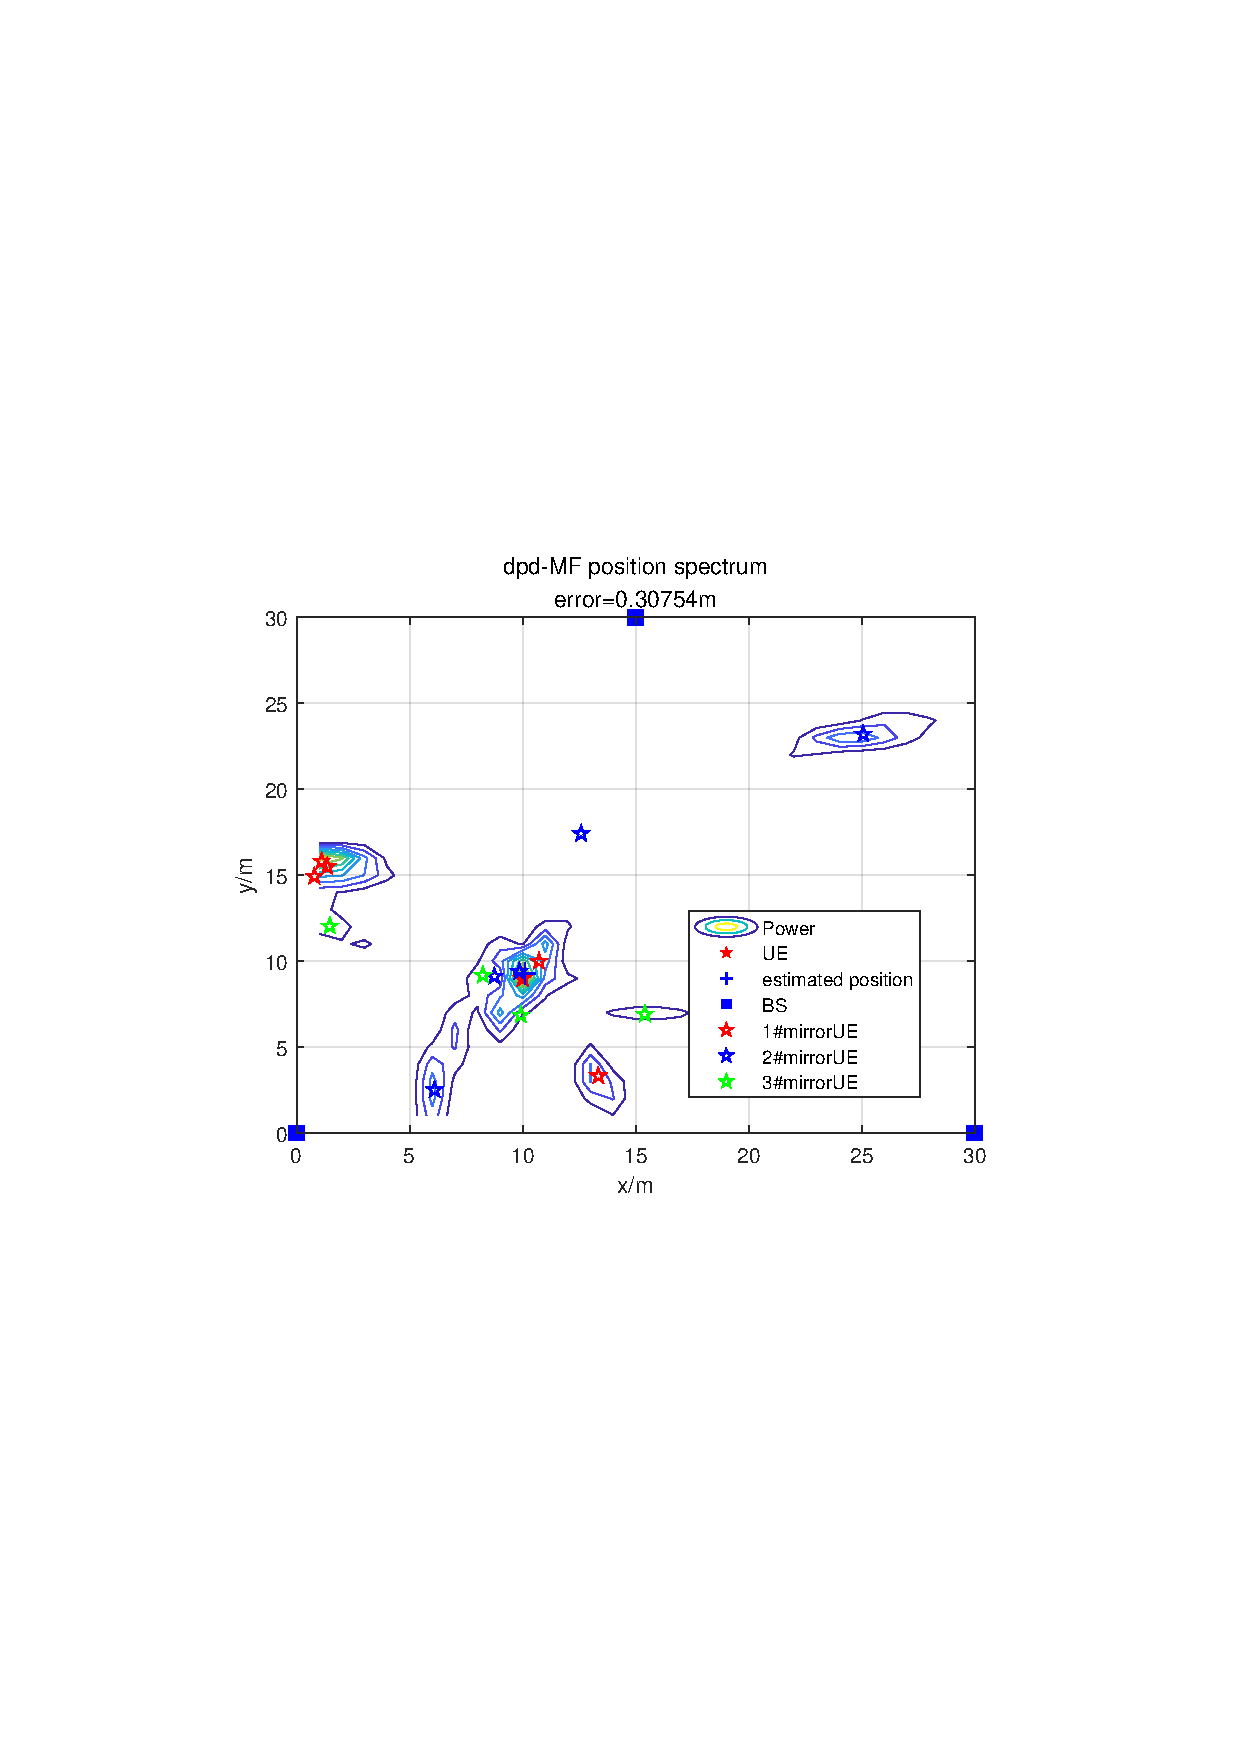
\includegraphics[width=0.5\textwidth]{figures/dpd-MFspectrum.pdf}}
  \centering
\caption{the dpd-MF position spectrum, SNR=20dB, $\Delta\tau_{min}=$1ns, $\Delta\theta_{min}=1^\circ$. The hollow pentacles (three kinds of colors) denote the 'Mirror UE' of three BSs respectively, the same bellow.}\label{dpd-MFspectrum}
\end{figure}
\begin{figure}[t]
  \centerline{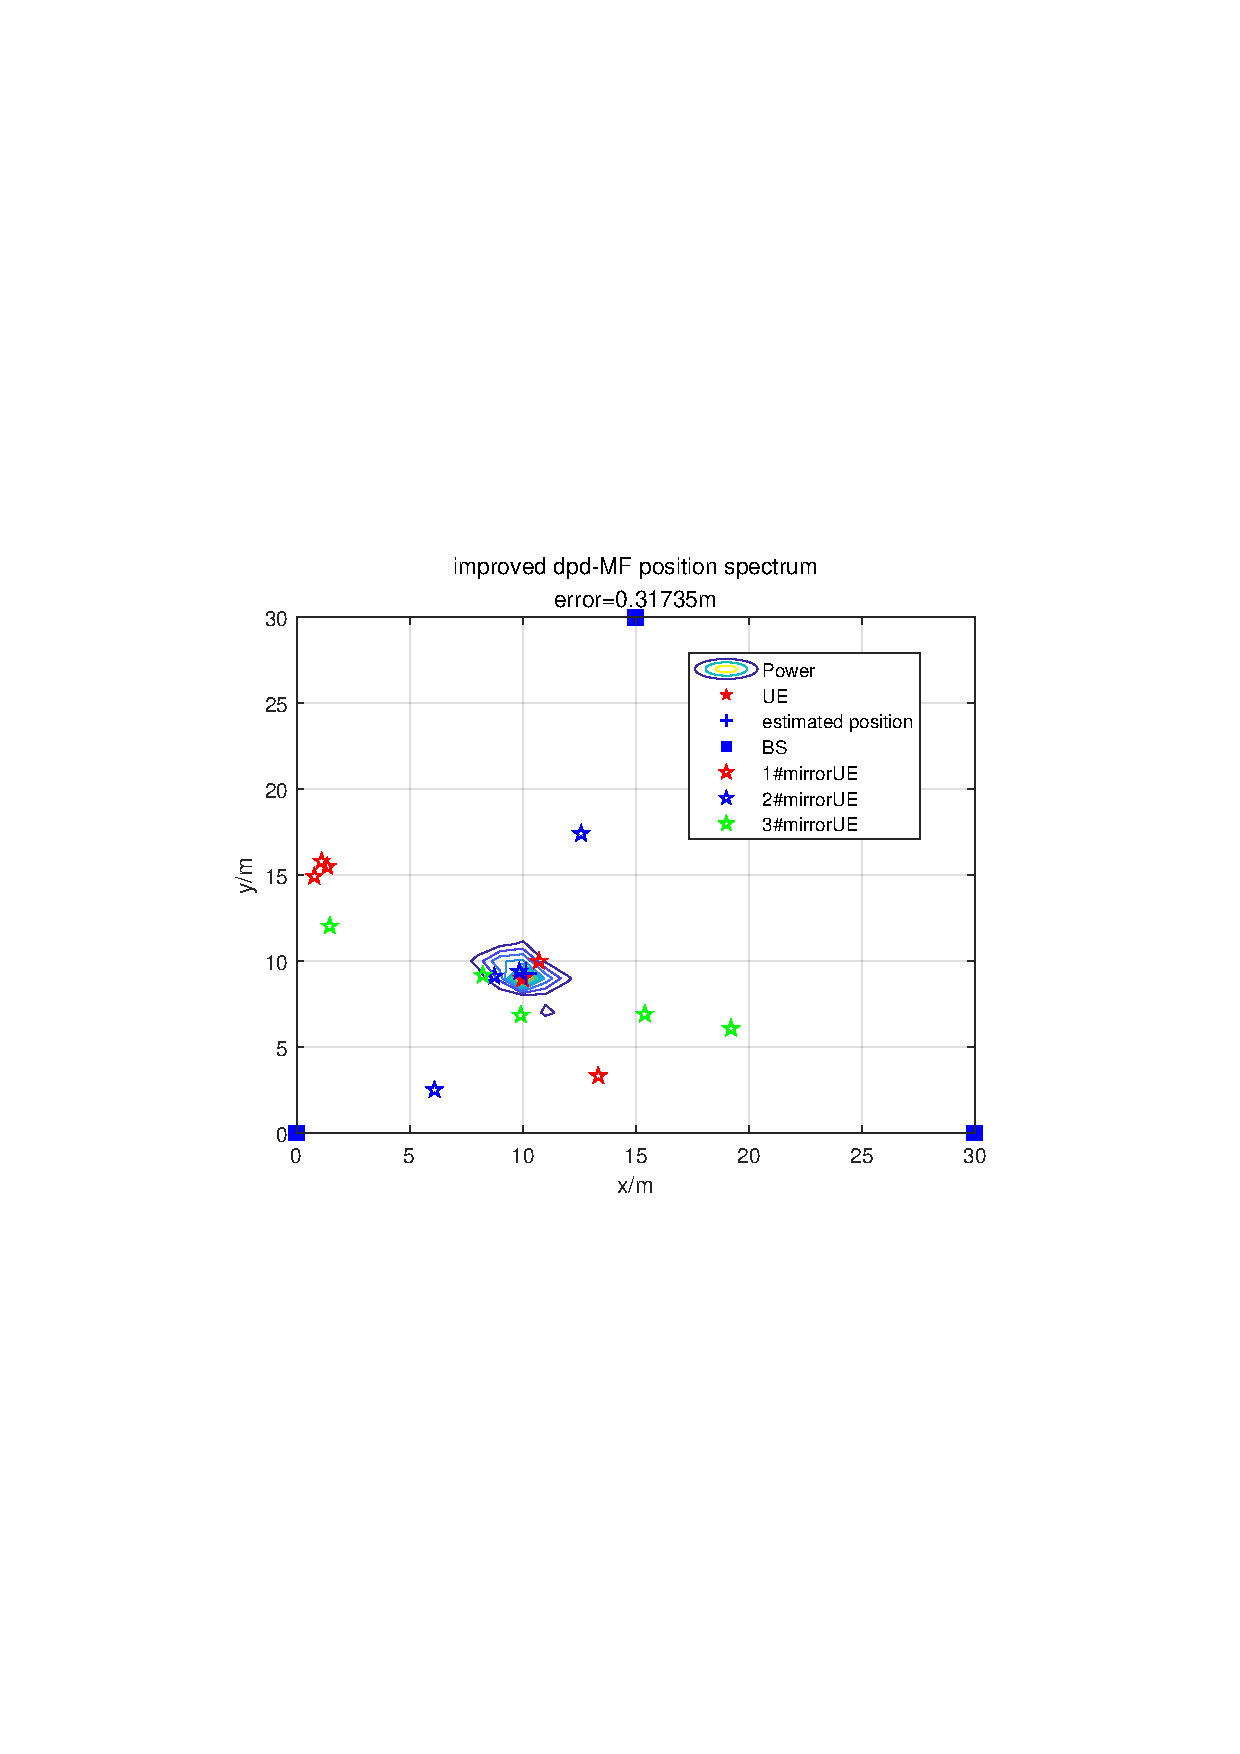
\includegraphics[width=0.5\textwidth]{figures/IprVdpd-MFspectrum.pdf}}
  \centering
\caption{the improved dpd-MF spectrum}\label{IprVdpd-MFspectrum}
\end{figure}
\section{Conclusion}
\label{sec:conclusion}
conclusion

% \appendices
% \section{Proof of the First  Equation}
% Appendix one text goes here.

% you can choose not to have a title for an appendix
% if you want by leaving the argument blank
% \section{}
% Appendix two text goes here.

%\section*{Acknowledgment}
%The authors would like to thank...



\balance
\bibliographystyle{IEEEtran}

\bibliography{refs}



\end{document}


